% 图 44.3 —— 由 `checks/emit_hand.py` 自动拼出（probe 精测 + prims2 图元分解）
%%
% ⚠ 这是**稿子不是成品**：跑 `checks/checkhand.py 44.3` 看指标 + 看叠合图。
%%
%% ⚠ 待核：
%   · 本图 probe 报出阴影族 1 个 —— **本脚本不生成阴影**（要照原书手写）；prims2 的 strokes 里可能含阴影线，核对时留意别画重
%   · 可疑字形 1 项（空心圈 ⊙ 常被认成字母 o）—— 见文件末
%%
\documentclass[12pt]{standalone}
\usepackage{fontspec}
\setsansfont{Arial}
\newfontfamily\mfallback{DejaVu Sans}
\usepackage{tikz}
\begin{document}
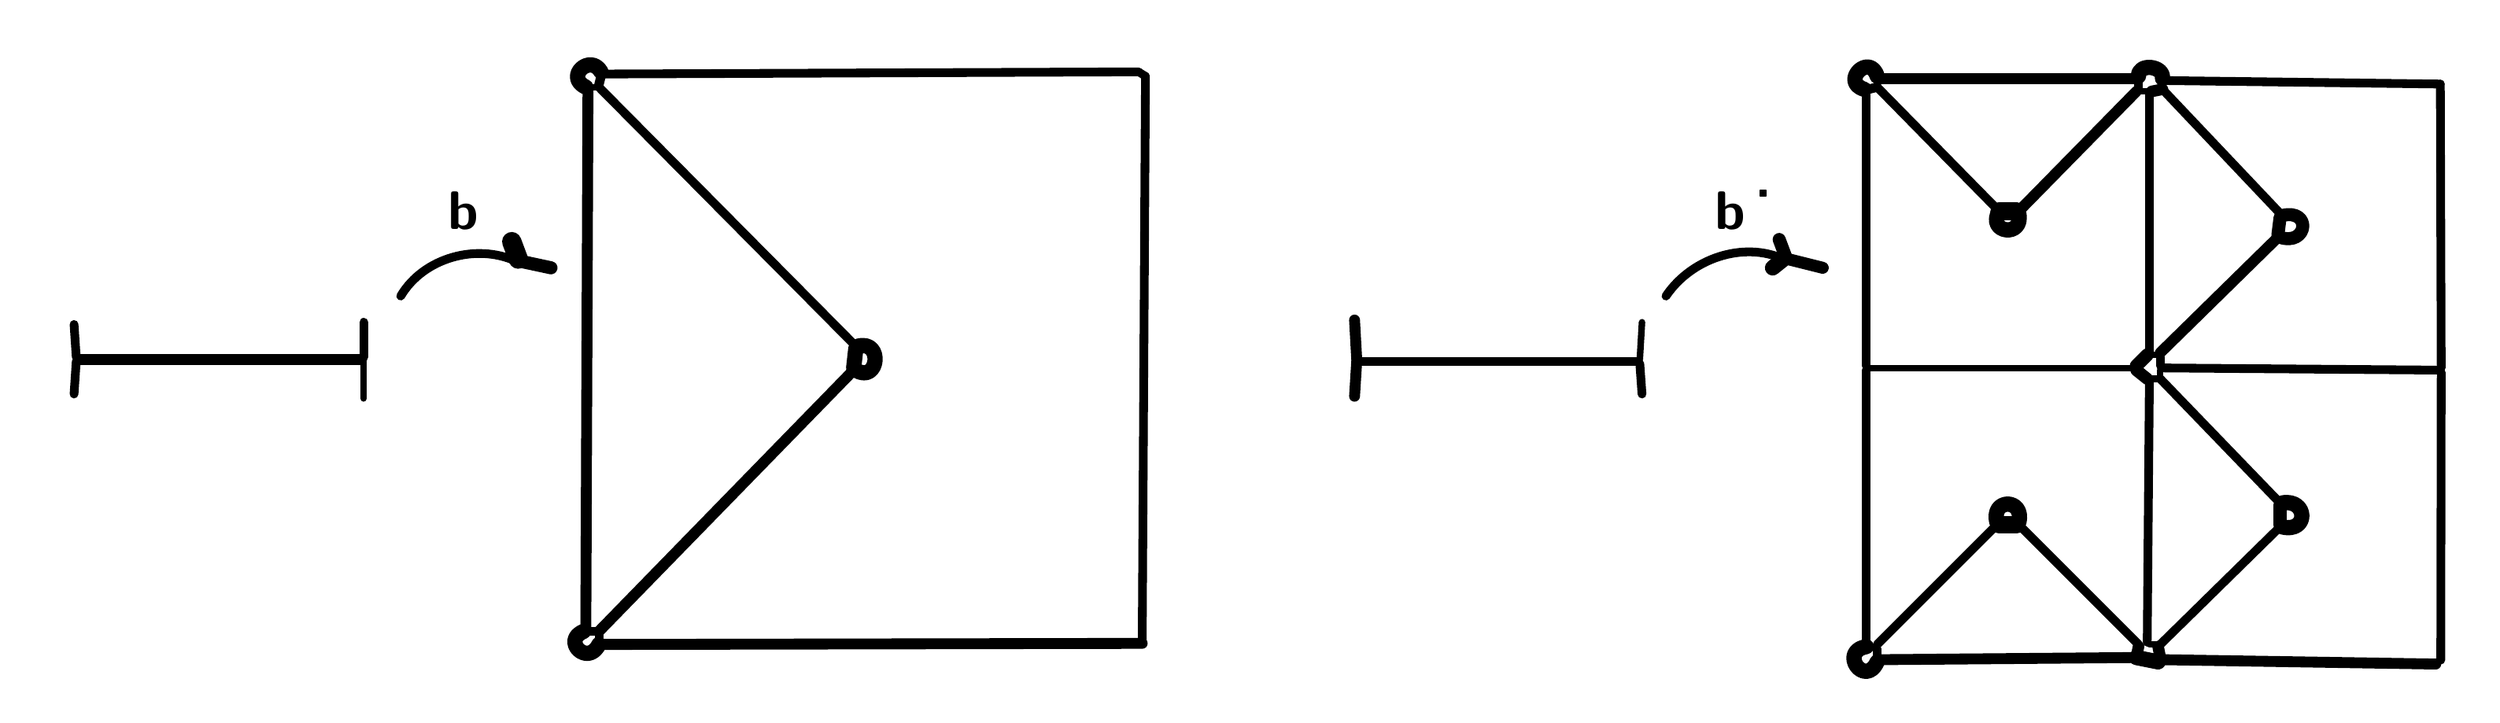
\begin{tikzpicture}[x=1pt, y=-1pt, line width=8.9pt, line cap=round, line join=round]

  %% ════ 直线段（prims2 的 strokes）════
  \draw[line width=8.9pt] (225.0,101.0) -- (228.0,109.0);
  \draw[line width=3.0pt] (852.0,27.0) -- (852.0,30.0);
  \draw[line width=5.0pt] (259.0,279.0) -- (260.0,31.0);
  \draw[line width=4.0pt] (24.0,171.0) -- (25.0,156.0);
  \draw[line width=4.0pt] (744.0,171.0) -- (743.0,157.0);
  \draw[line width=4.0pt] (265.0,281.0) -- (265.0,285.0);
  \draw[line width=4.0pt] (847.0,286.0) -- (847.0,160.0);
  \draw[line width=5.5pt] (976.0,164.0) -- (971.0,160.0);
  \draw[line width=5.0pt] (156.0,155.0) -- (26.0,155.0);
  \draw[line width=4.0pt] (976.0,285.0) -- (977.0,165.0);
  \draw[line width=4.0pt] (265.0,30.0) -- (383.0,149.0);
  \draw[line width=5.0pt] (853.0,26.0) -- (971.0,26.0);
  \draw[line width=4.0pt] (260.0,280.0) -- (264.0,280.0);
  \draw[line width=4.0pt] (983.0,159.0) -- (1110.0,160.0);
  \draw[line width=3.0pt] (848.0,287.0) -- (851.0,287.0);
  \draw[line width=4.0pt] (977.0,152.0) -- (977.0,33.0);
  \draw[line width=6.0pt] (976.0,153.0) -- (971.0,158.0);
  \draw[line width=5.0pt] (613.0,155.0) -- (612.0,137.0);
  \draw[line width=4.0pt] (1111.0,159.0) -- (1110.6,28.6);
  \draw[line width=4.0pt] (1110.6,28.6) -- (984.0,27.0);
  \draw[line width=3.0pt] (978.0,164.0) -- (981.0,164.0);
  \draw[line width=7.0pt] (981.0,294.0) -- (971.0,292.0);
  \draw[line width=3.0pt] (977.0,286.0) -- (980.0,286.0);
  \draw[line width=3.0pt] (848.0,159.0) -- (970.0,159.0);
  \draw[line width=5.0pt] (266.0,286.0) -- (514.5,285.5);
  \draw[line width=4.0pt] (514.5,285.5) -- (516.0,25.0);
  \draw[line width=3.8pt] (516.0,25.0) -- (512.8,23.0);
  \draw[line width=4.0pt] (512.8,23.0) -- (267.0,24.0);
  \draw[line width=3.0pt] (978.0,153.0) -- (981.0,153.0);
  \draw[line width=6.0pt] (807.0,100.0) -- (810.0,108.0);
  \draw[line width=3.0pt] (743.0,155.0) -- (744.0,138.0);
  \draw[line width=4.3pt] (852.0,30.0) -- (848.0,31.0);
  \draw[line width=4.0pt] (852.0,30.0) -- (908.0,87.0);
  \draw[line width=3.0pt] (983.0,28.0) -- (983.0,31.0);
  \draw[line width=3.0pt] (982.0,163.0) -- (982.0,160.0);
  \draw[line width=5.0pt] (613.0,156.0) -- (612.0,172.0);
  \draw[line width=8.0pt] (916.0,87.0) -- (908.0,87.0);
  \draw[line width=7.0pt] (383.0,150.0) -- (382.0,159.0);
  \draw[line width=4.0pt] (972.0,286.0) -- (917.0,231.0);
  \draw[line width=3.0pt] (976.0,32.0) -- (973.0,32.0);
  \draw[line width=4.0pt] (1037.0,232.0) -- (982.0,286.0);
  \draw[line width=5.3pt] (978.0,32.0) -- (983.0,31.0);
  \draw[line width=4.0pt] (157.0,138.0) -- (157.0,154.0);
  \draw[line width=4.0pt] (972.0,27.0) -- (972.0,31.0);
  \draw[line width=5.0pt] (971.0,32.0) -- (917.0,87.0);
  \draw[line width=6.0pt] (1037.0,222.0) -- (1037.0,231.0);
  \draw[line width=7.1pt] (804.0,113.0) -- (809.0,109.0);
  \draw[line width=5.0pt] (853.0,293.0) -- (971.0,292.0);
  \draw[line width=8.0pt] (908.0,231.0) -- (916.0,231.0);
  \draw[line width=5.0pt] (1035.0,100.0) -- (982.0,152.0);
  \draw[line width=4.0pt] (982.0,164.0) -- (1037.0,221.0);
  \draw[line width=4.3pt] (266.0,25.0) -- (265.0,29.0);
  \draw[line width=3.0pt] (157.0,156.0) -- (157.0,173.0);
  \draw[line width=5.0pt] (983.0,293.0) -- (1108.5,295.0);
  \draw[line width=2.9pt] (1108.5,295.0) -- (1110.8,293.2);
  \draw[line width=4.0pt] (1110.8,293.2) -- (1111.0,161.0);
  \draw[line width=4.0pt] (983.0,31.0) -- (1037.0,88.0);
  \draw[line width=5.5pt] (811.0,109.0) -- (827.0,113.0);
  \draw[line width=4.0pt] (847.0,32.0) -- (847.0,158.0);
  \draw[line width=4.0pt] (852.0,286.0) -- (907.0,231.0);
  \draw[line width=4.0pt] (614.0,156.0) -- (742.0,156.0);
  \draw[line width=3.0pt] (264.0,30.0) -- (261.0,30.0);
  \draw[line width=6.0pt] (229.0,110.0) -- (243.0,113.0);
  \draw[line width=4.0pt] (25.0,154.0) -- (24.0,139.0);
  \draw[line width=4.0pt] (852.0,292.0) -- (852.0,288.0);
  \draw[line width=5.3pt] (971.0,292.0) -- (972.0,287.0);
  \draw[line width=6.0pt] (1037.0,90.0) -- (1036.0,98.0);
  \draw[line width=4.0pt] (982.0,158.0) -- (982.0,154.0);
  \draw[line width=5.3pt] (982.0,292.0) -- (981.0,287.0);
  \draw[line width=5.0pt] (265.0,280.0) -- (382.0,160.0);

  %% ════ 曲线（prims2 的 curves —— 三段式，坐标同为 (y,x)）════
  \draw[line width=7.0pt] (1038.0,221.0) .. controls (1049.7,218.9) and (1050.3,234.9) .. (1038.0,232.0);
  \draw[line width=7.0pt] (384.0,149.0) .. controls (395.7,146.0) and (393.4,166.4) .. (383.0,160.0);
  \draw[line width=7.0pt] (852.0,25.0) .. controls (848.5,14.0) and (835.0,27.5) .. (846.0,31.0);
  \draw[line width=4.0pt] (174.0,126.0) .. controls (184.5,108.2) and (209.0,101.7) .. (227.0,110.0);
  \draw[line width=7.0pt] (983.0,26.0) .. controls (983.7,20.1) and (971.7,18.9) .. (972.0,25.0);
  \draw[line width=7.0pt] (917.0,230.0) .. controls (919.9,218.8) and (904.0,218.6) .. (907.0,230.0);
  \draw[line width=7.0pt] (847.0,287.0) .. controls (834.1,289.3) and (846.4,306.1) .. (852.0,294.0);
  \draw[line width=7.0pt] (265.0,286.0) .. controls (259.9,296.4) and (247.7,284.2) .. (258.0,280.0);
  \draw[line width=4.0pt] (809.0,109.0) .. controls (790.5,100.7) and (766.7,108.6) .. (755.0,126.0);
  \draw[line width=7.0pt] (266.0,23.0) .. controls (261.1,14.4) and (249.1,25.3) .. (259.0,30.0);
  \draw[line width=7.0pt] (917.0,88.0) .. controls (919.4,99.4) and (902.1,97.1) .. (908.0,87.0);
  \draw[line width=6.0pt] (1038.0,89.0) .. controls (1051.6,85.7) and (1049.8,103.1) .. (1037.0,99.0);

  %% ════ 标签（probe 直接给的 \node 行）════
  %% ⚠ 全部补了 fill=white：文字在最上层，否则与曲线交叉干扰
     \node[anchor=center,inner sep=0pt,fill=white,font=\fontsize{29.3}{36.6}\selectfont] at (202.7,86.7) {\textsf{\textbf{\textit{b}}}};   % box(193,75,17,21)
     \node[anchor=center,inner sep=0pt,fill=white,font=\fontsize{29.3}{36.6}\selectfont] at (784.7,86.7) {\textsf{\textbf{\textit{b}}}};   % box(775,75,17,21)
     \node[anchor=center,inner sep=0pt,fill=white,font=\fontsize{44.4}{55.5}\selectfont] at (799.8,78.9) {\textsf{\textbf{.}}};   % box(794,75,5,7)

  % 钉死画布：否则超出的图元/控制点会把页面撑大，1:1 回比就失准
  \pgfresetboundingbox
  \path[use as bounding box] (0,0) rectangle (1128,312);
\end{tikzpicture}
\end{document}

% ⚠ 待核清单（probe 拿不准，人眼过一遍）：
%   · 未识别/跳过：⑤ 跳过/未识别的字形
